\documentclass[tikz,border=12pt]{standalone}
\usepackage[T1]{fontenc}
\usepackage{mathpazo}
\usepackage{amsmath,amssymb}
\usetikzlibrary{arrows.meta, calc, positioning}

\definecolor{stblue}{HTML}{7B97AD}
\definecolor{rwgold}{HTML}{B8995E}
\definecolor{sage}{HTML}{7A9A7E}
\definecolor{dkbrown}{HTML}{3D3530}
\definecolor{wmgray}{HTML}{7B7067}
\definecolor{cream}{HTML}{F9F6F0}
\definecolor{border}{HTML}{D4C9B8}
\definecolor{terracotta}{HTML}{C47A6A}
\definecolor{lavender}{HTML}{907EA0}

\begin{document}
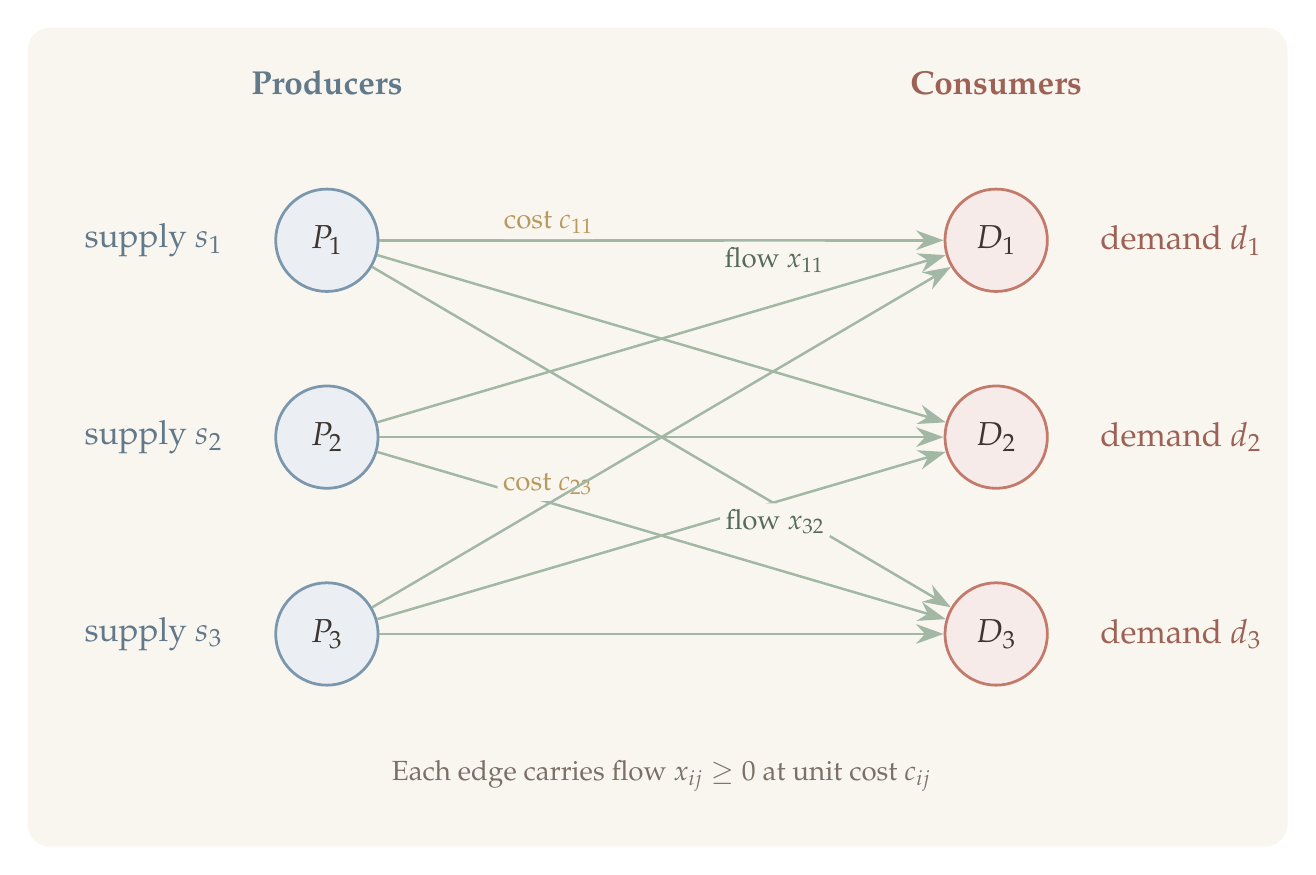
\begin{tikzpicture}[
    >={Stealth[length=3.5mm, width=2.5mm]},
    every node/.style={text=dkbrown},
  ]

  % Background
  \fill[cream, rounded corners=8pt] (-3.8,-5.2) rectangle (12.2,5.2);

  % --- Column headers ---
  \node[font=\large\bfseries, text=stblue!80!black] at (0,4.5) {Producers};
  \node[font=\large\bfseries, text=terracotta!80!black] at (8.5,4.5) {Consumers};

  % --- Producer nodes (left) ---
  \node[circle, fill=stblue!15, draw=stblue, line width=1pt,
        minimum size=1.3cm, font=\large\bfseries] (P1) at (0, 2.5) {$P_1$};
  \node[circle, fill=stblue!15, draw=stblue, line width=1pt,
        minimum size=1.3cm, font=\large\bfseries] (P2) at (0, 0)   {$P_2$};
  \node[circle, fill=stblue!15, draw=stblue, line width=1pt,
        minimum size=1.3cm, font=\large\bfseries] (P3) at (0,-2.5) {$P_3$};

  % --- Consumer nodes (right) ---
  \node[circle, fill=terracotta!15, draw=terracotta, line width=1pt,
        minimum size=1.3cm, font=\large\bfseries] (D1) at (8.5, 2.5) {$D_1$};
  \node[circle, fill=terracotta!15, draw=terracotta, line width=1pt,
        minimum size=1.3cm, font=\large\bfseries] (D2) at (8.5, 0)   {$D_2$};
  \node[circle, fill=terracotta!15, draw=terracotta, line width=1pt,
        minimum size=1.3cm, font=\large\bfseries] (D3) at (8.5,-2.5) {$D_3$};

  % --- Supply labels (left of producers) ---
  \node[font=\large, text=stblue!80!black, anchor=east] at (-1.2, 2.5) {supply $s_1$};
  \node[font=\large, text=stblue!80!black, anchor=east] at (-1.2, 0)   {supply $s_2$};
  \node[font=\large, text=stblue!80!black, anchor=east] at (-1.2,-2.5) {supply $s_3$};

  % --- Demand labels (right of consumers) ---
  \node[font=\large, text=terracotta!80!black, anchor=west] at (9.7, 2.5) {demand $d_1$};
  \node[font=\large, text=terracotta!80!black, anchor=west] at (9.7, 0)   {demand $d_2$};
  \node[font=\large, text=terracotta!80!black, anchor=west] at (9.7,-2.5) {demand $d_3$};

  % --- Edge style ---
  \tikzset{
    route/.style={->, sage!70, line width=0.9pt},
    costlbl/.style={font=\normalsize, text=rwgold, fill=cream,
                    inner sep=2pt, rounded corners=2pt},
    flowlbl/.style={font=\normalsize, text=sage!70!black, fill=cream,
                    inner sep=2pt, rounded corners=2pt},
  }

  % --- Edges (all 9 routes) with inline labels on select edges ---

  % P1 -> D1: annotated with cost and flow
  \draw[route] (P1) -- (D1)
    node[costlbl, pos=0.3, above] {cost $c_{11}$}
    node[flowlbl, pos=0.7, below] {flow $x_{11}$};
  % P1 -> D2, D3
  \draw[route] (P1) -- (D2);
  \draw[route] (P1) -- (D3);

  % P2 -> D1, D2
  \draw[route] (P2) -- (D1);
  \draw[route] (P2) -- (D2);
  % P2 -> D3: annotated with cost (label near P2 side to avoid crossing)
  \draw[route] (P2) -- (D3)
    node[costlbl, pos=0.30, above] {cost $c_{23}$};

  % P3 -> D1
  \draw[route] (P3) -- (D1);
  % P3 -> D2: annotated with flow (label near D2 side to avoid crossing)
  \draw[route] (P3) -- (D2)
    node[flowlbl, pos=0.70, below] {flow $x_{32}$};
  % P3 -> D3
  \draw[route] (P3) -- (D3);

  % --- General label for edges ---
  \node[font=\normalsize, text=wmgray, align=center] at (4.25, -4.3)
    {Each edge carries flow $x_{ij} \geq 0$ at unit cost $c_{ij}$};

\end{tikzpicture}
\end{document}
